\documentclass[12pt,letterpaper]{article}
\usepackage{graphicx,textcomp}
\usepackage{natbib}
\usepackage{setspace}
\usepackage{fullpage}
\usepackage{color}
\usepackage[reqno]{amsmath}
\usepackage{amsthm}
\usepackage{fancyvrb}
\usepackage{amssymb,enumerate}
\usepackage[all]{xy}
\usepackage{endnotes}
\usepackage{lscape}
\newtheorem{com}{Comment}
\usepackage{float}
\usepackage{hyperref}
\newtheorem{lem} {Lemma}
\newtheorem{prop}{Proposition}
\newtheorem{thm}{Theorem}
\newtheorem{defn}{Definition}
\newtheorem{cor}{Corollary}
\newtheorem{obs}{Observation}
\usepackage[compact]{titlesec}
\usepackage{dcolumn}
\usepackage{tikz}
\usetikzlibrary{arrows}
\usepackage{multirow}
\usepackage{xcolor}
\newcolumntype{.}{D{.}{.}{-1}}
\newcolumntype{d}[1]{D{.}{.}{#1}}
\definecolor{light-gray}{gray}{0.65}
\usepackage{url}
\usepackage{listings}
\usepackage{color}

\definecolor{codegreen}{rgb}{0,0.6,0}
\definecolor{codegray}{rgb}{0.5,0.5,0.5}
\definecolor{codepurple}{rgb}{0.58,0,0.82}
\definecolor{backcolour}{rgb}{0.95,0.95,0.92}

\lstdefinestyle{mystyle}{
	backgroundcolor=\color{backcolour},   
	commentstyle=\color{codegreen},
	keywordstyle=\color{magenta},
	numberstyle=\tiny\color{codegray},
	stringstyle=\color{codepurple},
	basicstyle=\footnotesize,
	breakatwhitespace=false,         
	breaklines=true,                 
	captionpos=b,                    
	keepspaces=true,                 
	numbers=left,                    
	numbersep=5pt,                  
	showspaces=false,                
	showstringspaces=false,
	showtabs=false,                  
	tabsize=2
}
\lstset{style=mystyle}
\newcommand{\Sref}[1]{Section~\ref{#1}}
\newtheorem{hyp}{Hypothesis}


\title{Exam 2-Darragh Kane O Toole-18431115 }
\date{Due: December 9th, 2022}
\author{Applied Stats/Quant Methods 1}


\begin{document}
	\maketitle
	\section*{Instructions}
	\begin{itemize}
		\item Please read carefully: You have from 09:00 Wednesday December 7 until 08:59
		Friday December 9 to complete the exam. Please export your answers as a single
		PDF file and include all code you produce in a supporting R file, which you will
		upload to Blackboard. The exam is open book; you can consult any materials you
		like. You must not collborate with or seek help from other students. In case
		of questions or technical difficulties, you can contact Professor Ziegler via email. You
		should write-up your answers in R and LaTeX as you would for a problem set. Please
		make sure to concisely number your answers so that they can be matched with the
		corresponding questions.
	\end{itemize}
	
	
	
	\vspace{.5cm}
	\section*{Question 1}
	\vspace{.25cm}
	\noindent 	
	Define and describe why the following four (4) terms are important to hypothesis testing
	and/or regression. You can earn full credit with just two or three sentences, but please be
	specific and thorough.
	 
	 \newpage
	\begin{enumerate}
		
		\item [(a)]
		Residuals- Residuals can be used to determine if variables are related by measuing the difference etween observed and fitted values.
		
		\vspace{1cm}
		\item [(b)]
		Categorical data- This a type of data that is representing a set of characteristics or traits,examples of this could be nationality or gender where there is a defined  amout of groups which you cna be assigned to. It has no order or rank.\\

		Dummy variables- These are when you use a categroical variable as a predictor in a regression to seperate a group to see if the effect varies within the groups characteristics. An example fo this could be that without rnak at a job considered better work leads to mre income but if a dummy variable is implemented it can show if this effect is true for managers and not managers adding insight to data.
		
		\vspace{1cm}
		\item [(c)]
		Test statistic- This is a statistic that sumarrises how much data is different from what would be expected to observe if the null hypothesis were true 
		\vspace{1cm}
		\item [(d)]
		Constituent term-This is at times also called "main effects" as in a multiple Regression are the variables which represent a portion of the effect.

		
	\end{enumerate}
	
	\newpage
	
	\section*{Question 2}
	\vspace{.25cm}
	\noindent 	Many of the wells used for drinking water in Bangladesh and other South Asian countries are contaminated with natural arsenic, affecting an estimated 100 million people. Arsenic is a cumulative poison, and exposure increases the risk of cancer and other diseases, with risks
	estimated to be proportional to exposure.\\
	We performed a regression analysis with the data to understand the factors that predict the arsenic level of 1000 households’ drinking water. Your outcome variable arsenic is a continuous measure of household i’s arsenic level in units of hundreds of micrograms per liter.\\
	We estimated models with the following inputs:\\
	• The distance (in kilometers/100) to the closest known commercial factory\\
	• Depth of respondent’s well (binary variable; deep=1, not deep=0)
\begin{figure}
\centering
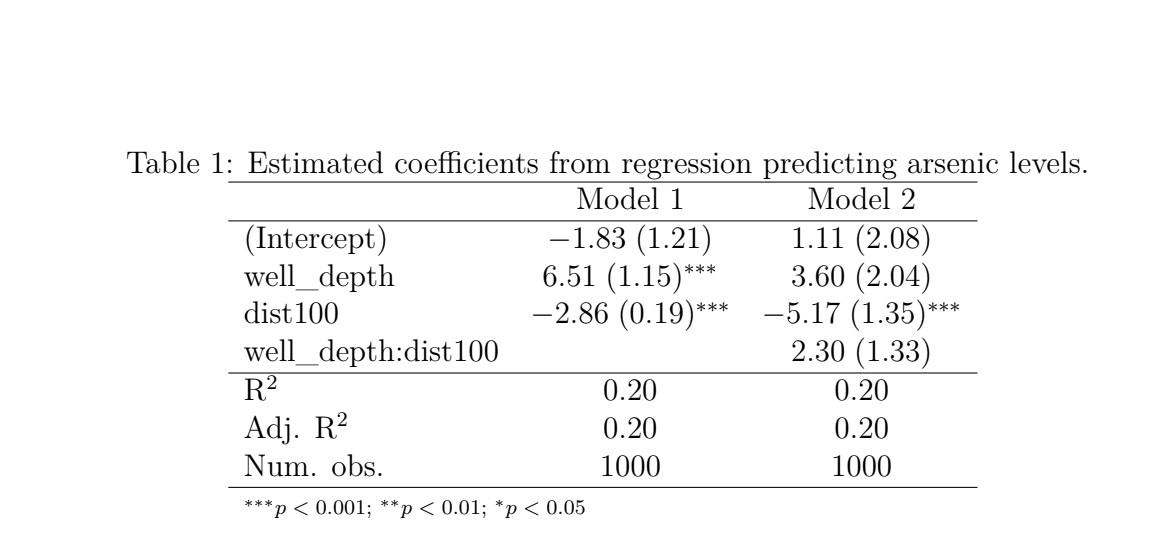
\includegraphics[width=0.7\linewidth]{Q2}
\caption{}
\label{fig:q2}
\end{figure}


	
	
	\vspace{.5cm}
	
	
	\vspace{.5cm}
	\begin{enumerate}
		\item [(a)] First, we successfully estimated an additive model with well depth and distance to
		the nearest factory as the two predictors of a household’s arsenic level. The estimated
		coefficients are found in the first column of the table above. Interpret the estimated
		coefficients for the intercept and each predictor.\\
		
		The intercept indicates there is rarely arsenic in the water overall as its a negative number.\\
		Based of the table well depth in the additive model leads to(6.51) increased arsenice in the water while distance to the well (-2.86) decreased the arsenic in the water. 
		
		

		
		\item [(b)]  Does the coefficient estimate for the closest known factory vary based on whether or not
		a house has a deep well? If so, change your interpretation of the estimated coefficients
		in part (a) to conform with the interactive model in column 2 of the table above. What
		is the appropriate test to determine whether we should model the relationship between
		distance, well depth, and arsenic levels using an additive or interactive model? What
		information would you need to perform that test?\\
		
		A partial F test is an apropriate test to determine if an interactive model is apporriate to use in this data,If variance is constant the estimate is better with an interaction model. To do an a partial F test you need mean squares(treatement)/mean squares (error)
		
		
		
		\vspace{2cm}
		\item [(c)] Using the ‘preferred’ model from Part B, compute the average difference in arsenic
		levels between two households that have a deep well (=1), but one is closer to a factory
		(dist100 = 0.42) than the other (dist100 = 2.12).
		\vspace{7cm}
		\lstinputlisting[language=R, firstline=22, lastline=25]{Exm2.R}  
		
		
	\end{enumerate}  
	\newpage

	
	\section*{Question 3}
	\vspace{.25cm}
	\noindent 	This data set presents information on 33 lambs, of which 11 are ewe lambs, 11 are wether
	lambs, and 11 are ram lambs. These lambs grazed together in the same pasture and were
	treated similarly in all ways. The variables of interest are presented in the table below.
	\begin{figure}
	\centering
	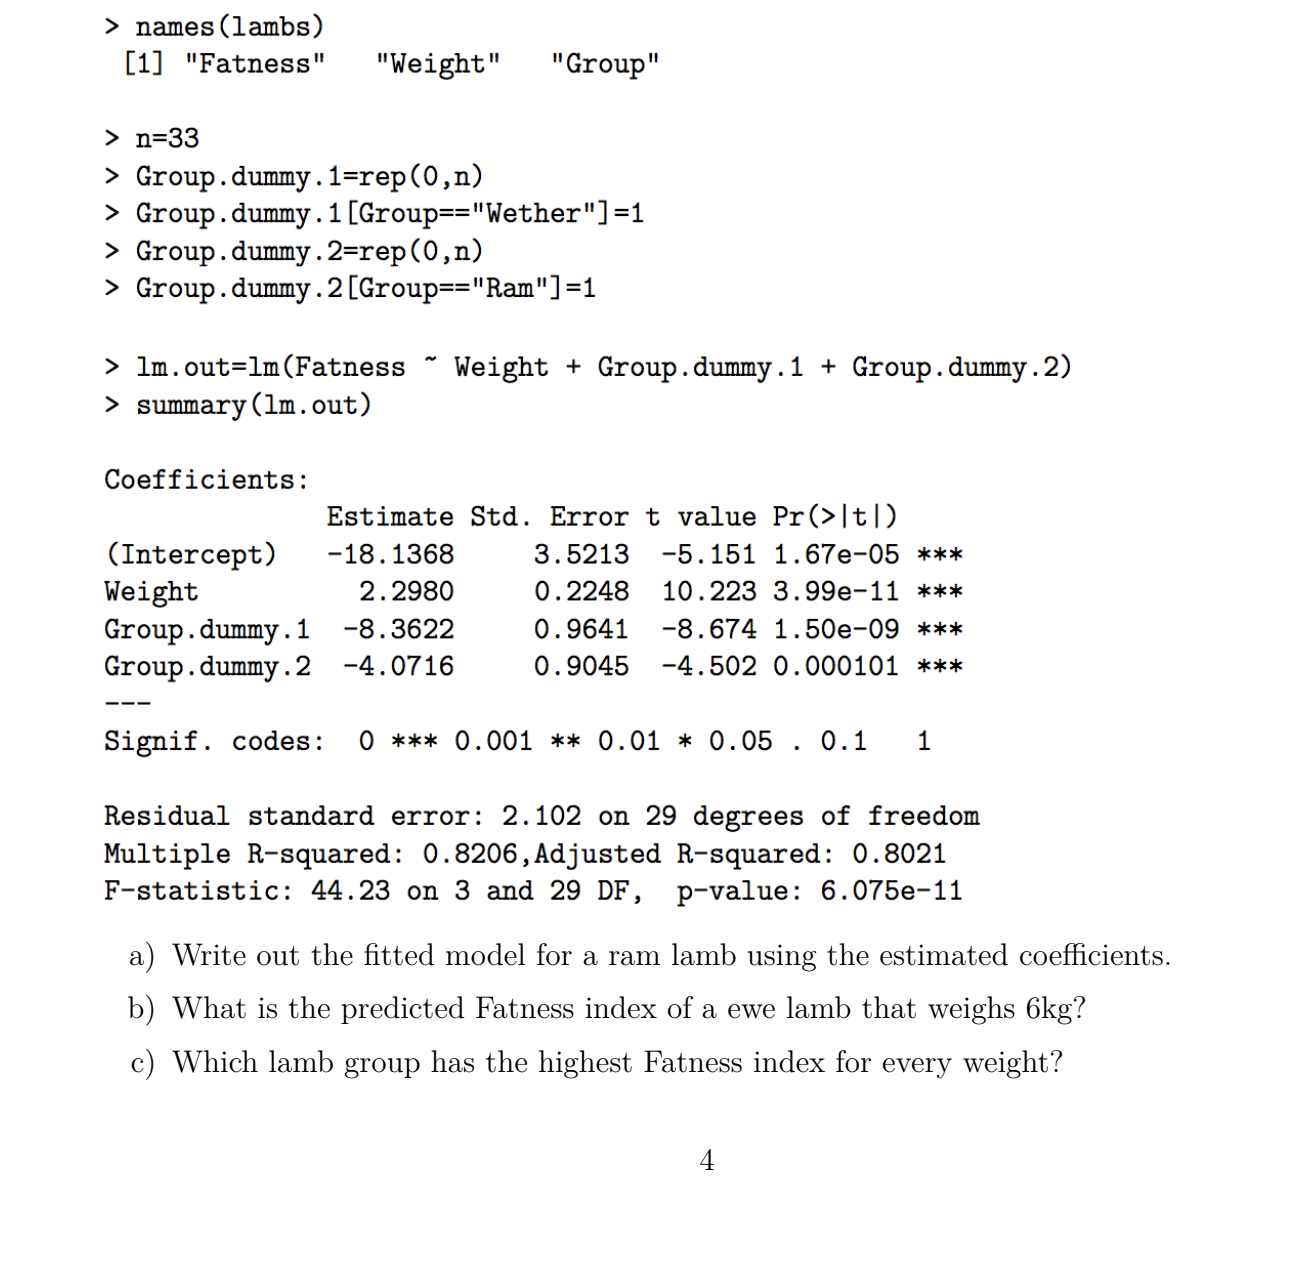
\includegraphics[width=0.7\linewidth]{Q3}
	\caption{}
	\label{fig:q3}
	\end{figure}
	
	
	
	
	\vspace{.5cm}
	
	
	\vspace{.5cm}
	\begin{enumerate}
	\lstinputlisting[language=R, firstline=31, lastline=32]{Exm2.R}  
	
	
	
	
	\item [(b)] ewe is 0 is neither Ram or wether so if boths dummy variable is set to 0 all theats left is ewe
		\lstinputlisting[language=R, firstline=35, lastline=37]{Exm2.R}  
	
	
	
	\vspace{2cm}
	\item [(c)] For all weights I set to 0 to remove bring the varibale as low as possible and comapare.
			\lstinputlisting[language=R, firstline=38, lastline=46]{Exm2.R}  
	
	
	\end{enumerate}  
	\newpage
	
	
	\section*{Question 4}
	\vspace{.25cm}
\begin{figure}[H]
\centering
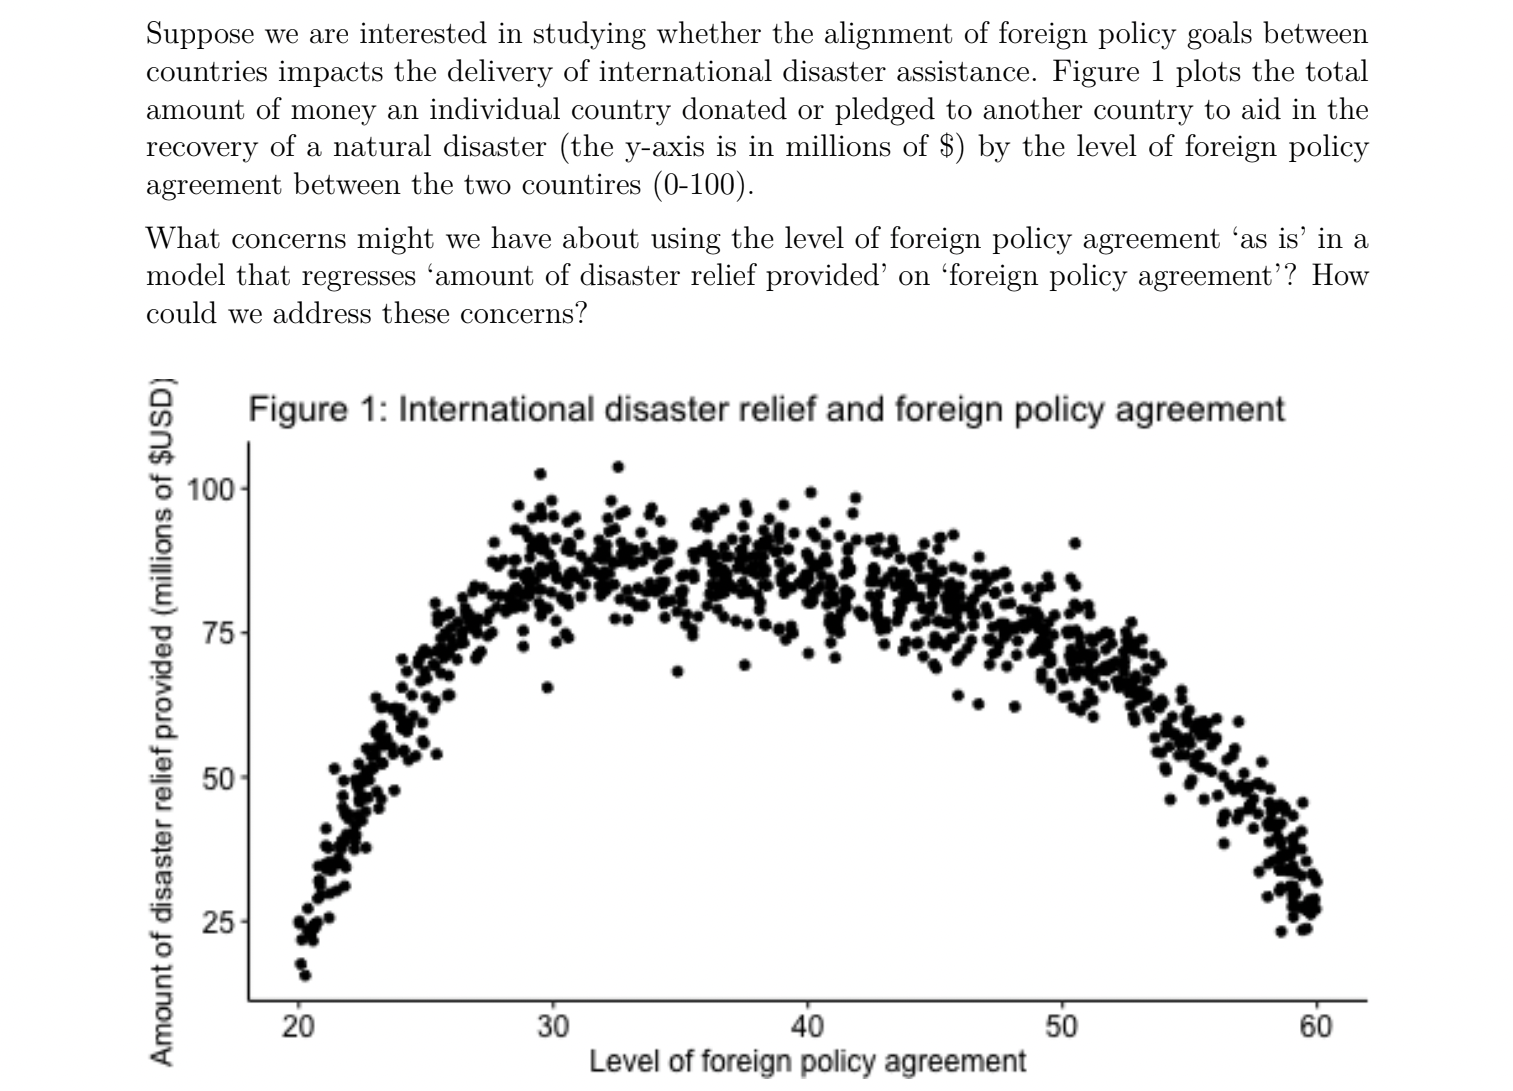
\includegraphics[width=0.7\linewidth]{Q4}
\caption{}
\label{fig:q4}
\end{figure}
	\begin{enumerate}
	\item [(a)] 
	A concern about ths model is the shape of the relationship which is in this case not linear. To resolve this you would square route the variable and the graph would become linear. This 
	
	\end{enumerate}  
		\section*{Question 5}
	\vspace{.25cm}
	\noindent Please select the most appropriate option to correctly answer each question.\\
	
	Which of the following plots is used to check for normality in the assumptions of linear
	regression?\\
	1. Scatterplot between residuals and X\\
	2. Scatterplot between residuals and Y\\
	3. Histogram of Y\\
	4. QQ plot of residuals-ANSWER\\
	
	The coefficients in an ordinary least squares regression model .\\
	1. are generalized additive estimates\\
	2. are maximum likelihood estimates\\
	3. minimize the residual sum of squares-ANSWER\\
	4. maximize the regression sum of squares\\
	
	We can calculate our standard errors by taking the square root of the off-diagonal elements
	in our variance-covariance matrix.\\
	1. True-ANSWER\\
	2. False\\
	
	Suppose you are interested in knowing the different impact of age (continuous) by educational
	background (categorized as arts or science/engineering) on a job candidate’s potential salary
	(continuous). Which test or technique would you use?\\
	1. Simple bivariate linear regression model\\
	2. Additive (salary = age + education) regression model-ANSWER\\
	3. Interactive (salary = age * education) regression model\\
	4. Interactive (education = age * salary) regression model\\
	
	
	
	
	\vspace{.5cm}

		\section*{Question 6}
	\vspace{.25cm}
	\noindent 
\begin{figure}[H]
\centering
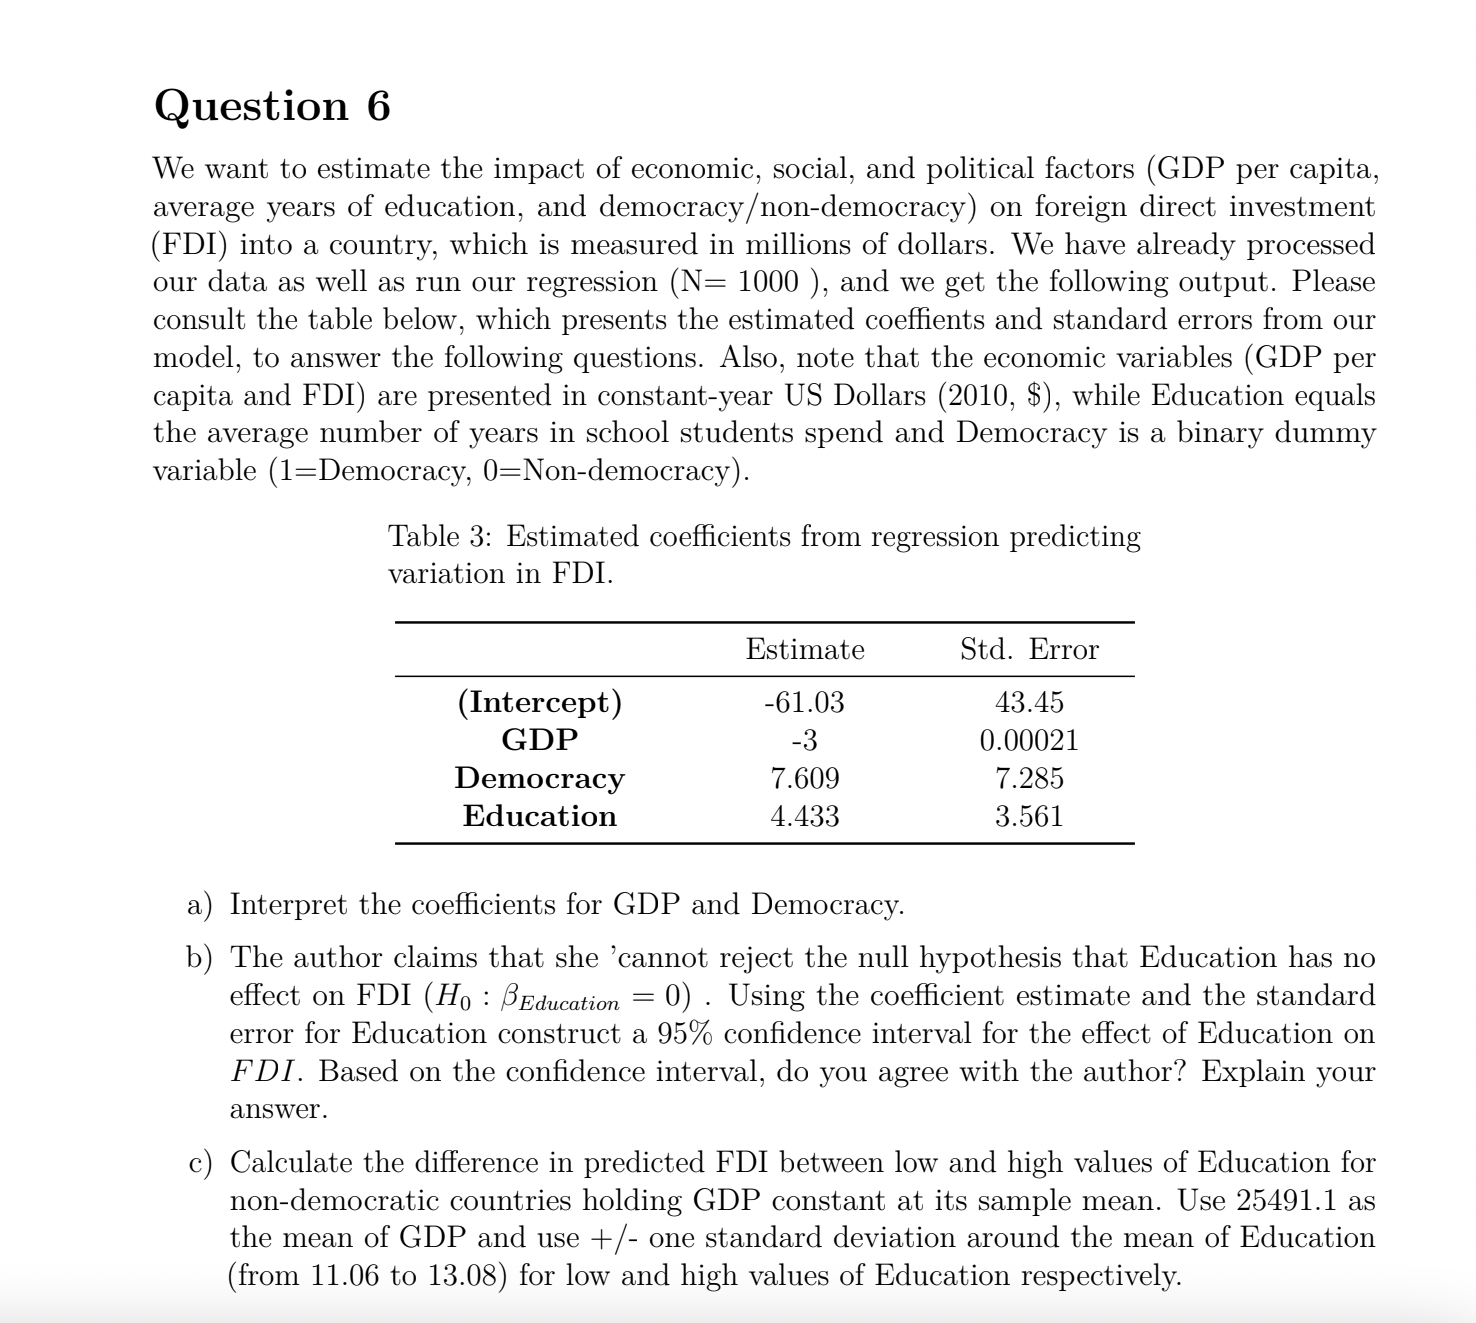
\includegraphics[width=0.7\linewidth]{Q6}
\caption{}
\label{fig:q6}
\end{figure}

	
	\vspace{.5cm}
	\begin{enumerate}
	\item [(a)] Interpret the coefficients for GDP and Democracy.\\
	GDP is related to a decrease in FDI(-3 coeffecient)\\
	Democracy is related to an increase in FDI(7.609)
	
	
	
	
	\item [(b)] The author claims that she ’cannot reject the null hypothesis that Education has no
	effect on FDI (H0 : BEducation = 0) . Using the coefficient estimate and the standard
	error for Education construct a 95% confidence interval for the effect of Education on
	F DI. Based on the confidence interval, do you agree with the author? Explain your
	answer.\\
	Given how wide the range is,it is unlikely in my view that the education has 
	no effect on FDI so I disagree with the Author and would rejec tthe Null hypothesis
	educations is a non zero effect on FDI
		\lstinputlisting[language=R, firstline=3, lastline=6]{Exm2.R}  
	
	
	
	\vspace{2cm}
	\item [(c)] Calculate the difference in predicted FDI between low and high values of Education for
	non-democratic countries holding GDP constant at its sample mean. Use 25491.1 as
	the mean of GDP and use +/- one standard deviation around the mean of Education
	(from 11.06 to 13.08) for low and high values of Education respectively.
			\lstinputlisting[language=R, firstline=11, lastline=16]{Exm2.R}  
	
	
	\end{enumerate}  
	
	
	
	
\end{document}
